\section{Software Design}

Each node in the FANS system has its software design outlined below. Simple system nodes with an algorithmic design
have their control flow described using state machine diagrams as an aid. Class diagrams are included for nodes that
use an object-oriented approach for their design.

\subsection{Sensor Data Collection System}

The sensor collection system will be programmed using the Python programming language for simplicity and its large
collection of libraries.

The structure of the program will be that of two continuous polling loops, running as separate processes to utilize the
CPU fully and get around the Global Interpreter Lock (GIL) of Python that prevents maximizing traditional thread
performance.

The first polling loop will be responsible for collecting sensor data continuously and placing it on a queue for the
other loop. It will collect data from all sensors, and that is its sole responsibility.

\begin{figure}[H]
    \centering
    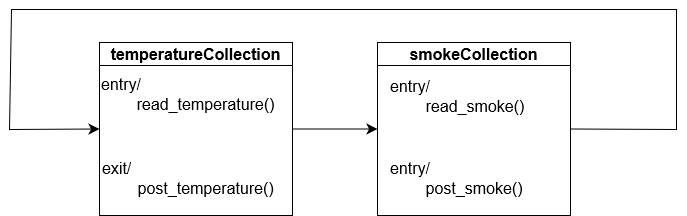
\includegraphics[width=\linewidth]{../assets/DataCollectionStateMachine.png}
    \caption{The polling loop for sensor data collection.}
\end{figure}

The second polling loop will be responsible for reading the sensor data from the shared queue and writing it to the
Firebase database. It will also be responsible for performing logical checks on this data to determine whether or not
there is an active fire emergency. It will update the emergency flag in the database whenever a sensor data measurement
is above the specified threshold, and also communicate the emergency over UDP to the notification system and alarm
system. Once all sensor data has been posted to the database, this loop will check for configuration updates in the
sensor data thresholds from the Firebase database and apply them to the next iteration.

\begin{figure}[H]
    \centering
    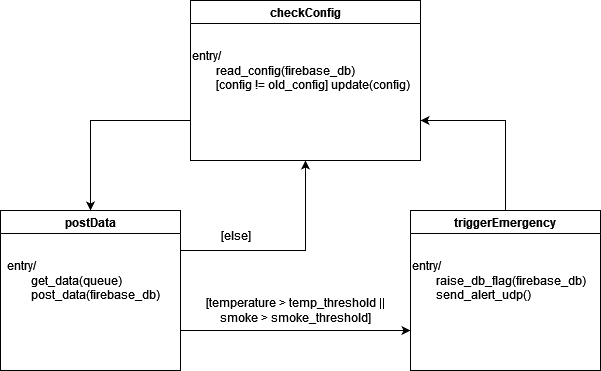
\includegraphics[width=\linewidth]{../assets/DataCollectionLogicLoop.png}
    \caption{State machine diagram for the second process of the sensor data collection system.}
\end{figure}

\subsection{Alarm System}

The alarm system will be programmed using the Python programming language, again for its simplicity. The alarm system
will be composed of one continuous loop, which waits to receive incoming UDP messages. When a UDP message signifying an
emergency is received, the alarm system will trigger both an alarm buzzer and flashing LED lights for an infinite
duration. The alarm response will be interrupted only when the system receives another UDP message signifying that the
emergency has ended. This behaviour is similar to a state machine, so the software will be created using the state
design pattern.

\begin{figure}[H]
    \centering
    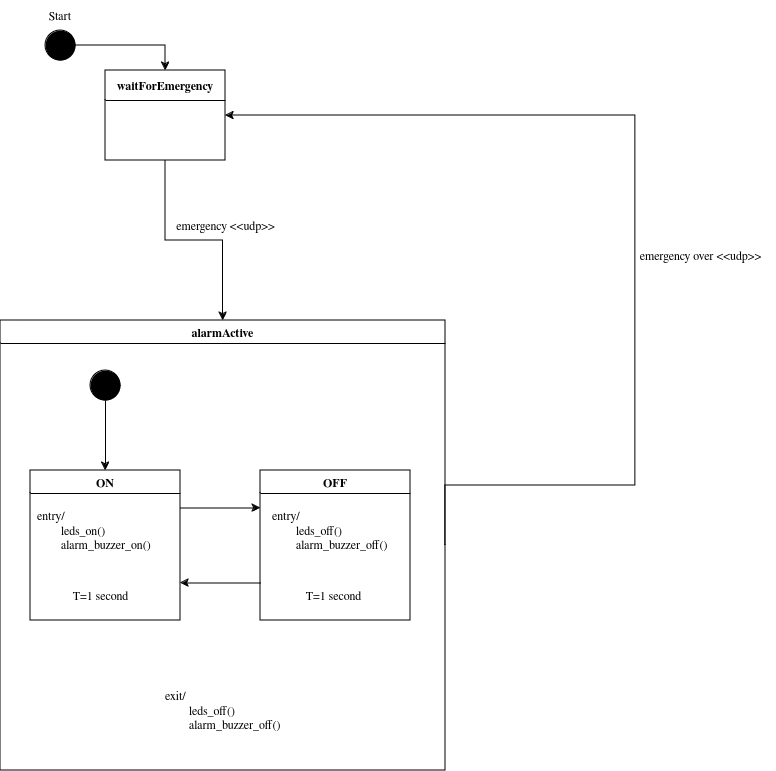
\includegraphics[width=\linewidth]{../assets/AlarmSystemStateMachine.png}
    \caption{State machine diagram for the alarm system node.}
\end{figure}

\subsection{Notification System}

The notification system will be written in the Python programming language, also due to its simplicity and availability
of libraries for sending email notifications \cite{python-email}. The notification system will listen for a UDP message
signifying an emergency, and then send out email and SMS notifications to all users in the Firebase database. Once a
UDP message signifying the end of the emergency is received, the system will send a followup email to all users that
the emergency has been resolved.

\begin{figure}[H]
    \centering
    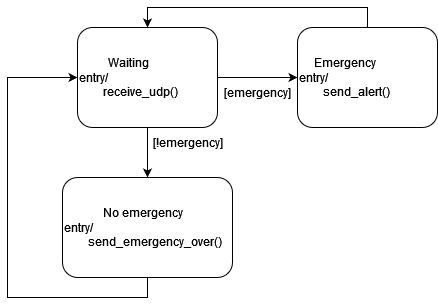
\includegraphics[width=4in]{../assets/NotificationSystemStateMachine.png}
    \caption{The state machine representing the primary functionality of the notification system.}
\end{figure}

The notification system will keep a local cache of user contact information as a backup for failing internet
connectivity. It will periodically update its local cache with any changes in the upstream Firebase database.

The notification system will also have locally stored email and SMS templates for notifications. These will be loaded
as "Templates", which provide an interface for easy customization and sending of notifications.

\begin{figure}[H]
    \centering
    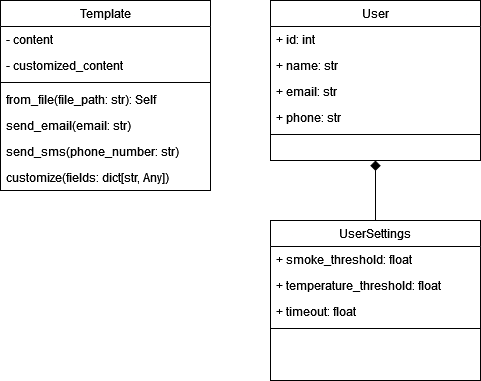
\includegraphics[width=3in]{../assets/NotificationSystemClassDiagram.png}
    \caption{Class diagram for the notification system node.}
\end{figure}

\subsection{Haptic Alarm System}

The haptic alarm wearable also has a very simple software design, and will be written in the Python programming
language. The program will continuously poll the Firebase database for changes in the emergency flag. Once the
emergency flag has been raised, the haptic alarm will begin to buzz on and off. During this time, it will continue
checking for changes in the emergency flag on the Firebase database. Once the emergency flag is lowered, the haptic
alarm will stop buzzing, signifying the end of the emergency.

\begin{figure}[H]
    \centering
    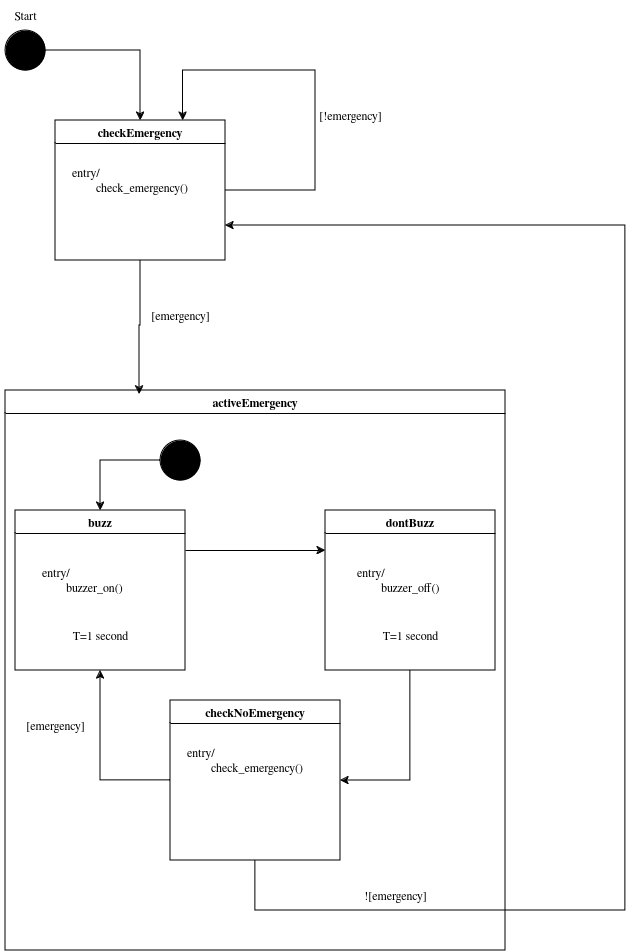
\includegraphics[width=4in]{../assets/HapticAlarmStateMachine.png}
    \caption{State machine diagram for the haptic alarm system node.}
\end{figure}
